\documentclass[a4paper]{leaflet}

\usepackage[T1]{fontenc}
\usepackage[utf8]{inputenc}
\usepackage[french]{babel}
\usepackage{rotating}
\usepackage{adjustbox}

\newcommand{\ei}{\textperiodcentered}
\begin{document}
\begin{titlepage}
  \title{
    Soutenance de thèse d'Emilie Buessler
    \date{16/12/2019} \\
    \textsc{Construction et Validation d'un Atlas Statistique 3D des Os Carpiens Humains.}\\[1cm]    
    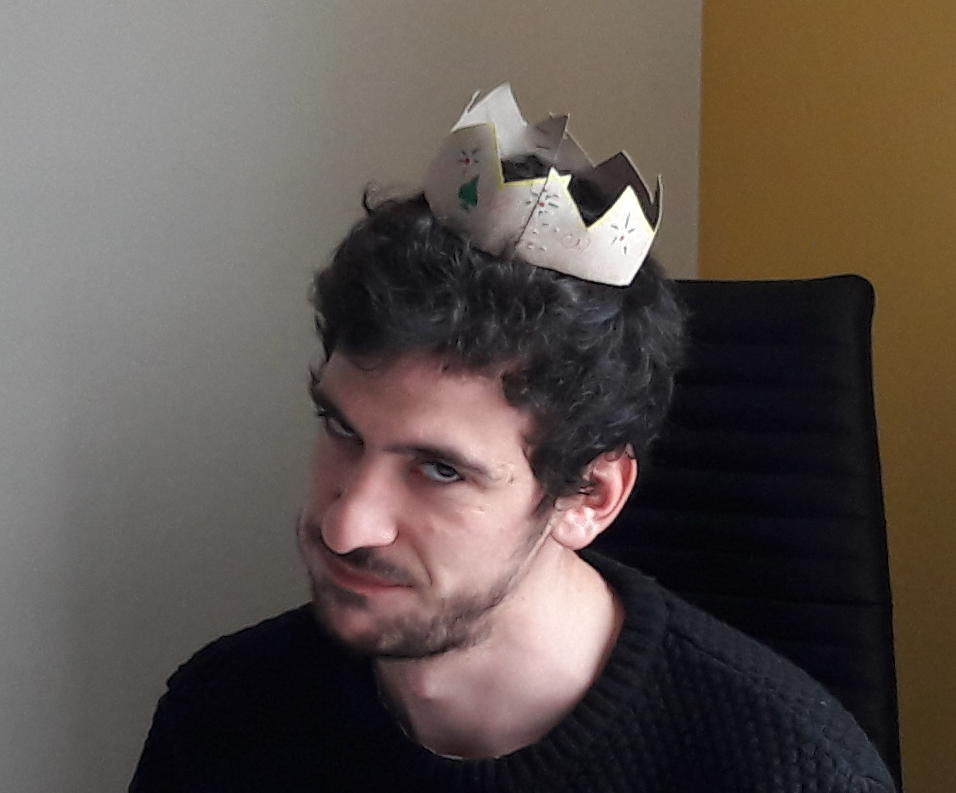
\includegraphics[width=0.5\textwidth]{crop} \\
 sous la direction de: \\
Lionel REVERET \\
Franck QUAINE \\
}
\end{titlepage}

\maketitle

\newpage
\section*{Résumé}
Le but de cette thèse est de permettre une capture anatomique fiable de la main humaine à partir d'une source vidéo, standard ou 3D, en s'appuyant sur un modèle biomécanique complet allant du poignet aux doigts, intégrant os, muscles, tendons et ligaments. Plusieurs modèles de la main existent déjà pour décrire la biomécanique des parties phalanges et métacarpienne, très peu ont été proposés pour la partie carpienne, aucun n'incluent les trois parties. Le fonctionnement complet de la main repose cependant sur une synergie de tous ces éléments. L'originalité scientifique du projet est donc de viser une modélisation complète, au-delà des modèles simplifiés utilisés en suivi automatique. Grâce à une collaboration internationale avec le département d'Orthopédie de Brown University (RI, USA), le projet a un accès privilégié à une source unique de données radiographiques. De plus, suite au projet EQUIPEX KINOVIS auquel participent UJF et INRIA, cet avantage expérimental sera prolongé par la récente mise en place d'une plateforme similaire d'analyse par rayons X du mouvement au LADAF (laboratoire d'Anatomie de l'UJF à la Faculté de Médecine). Par sa complexité et sa place au centre de l'activité humaine, la main reste un sujet scientifique majeur en biomécanique. Du fait de cette complexité, le développement de la connaissance scientifique dans ce domaine tend légitimement à se spécialiser sur certaines articulations. Dans le même temps, la recherche en informatique graphique a suscité le développement de solutions techniques sophistiquées en simulation physique pour améliorer le réalisme visuel des personnages de synthèse. La main fait partie de ces réalisations, avec un souci dans ce contexte de la représenter dans sa totalité. Le présent projet place donc l'ambition d'apporter à la biomécanique les avancées en simulation 3D, tout en ne se limitant pas à la qualité du réalisme visuel, mais en exigeant une validation exhaustive permise par un environnement expérimental novateur.
\section*{Résumé vulgarisé}
Savoir comment se placent les petits os de la main est une question compliquée car leur position dépend, entre autre, de celles de leurs voisins. Cependant, ça serait utile pour pouvoir, par exemple, les réparer (chirurgie, prothèses...). C'est ce qu'a fait Emilie pendant sa thèse, en utilisant des radios de main.

\section*{Déroulement de la soutenance}
La soutenance se déroule en plusieurs étapes:
\begin{itemize}
\item la soutenance:($\approx$ 45 min):
  le\ei la candidat\ei e présente de manière concise ses travaux.  \textbf{NE PAS APPLAUDIR À LA FIN DE LA PRÉSENTATION}.  Il est possible de partir à la fin de celle-ci, car souvent les questions sont très pointues et la durée peut être variable.
\item les questions du jury ($\approx$ 30 min, 1h):
  Le jury interroge le\ei la candidat\ei e sur ses travaux, sur la présentation et le manuscrit de thèse qu'il\ei elle leur aura envoyé auparavant.
\item la délibération ($\approx$ 1h):
  Le\ei la candidat\ei e peut souffler, pendant que le jury se réunit dans une pièce à part, afin de décider de l'obtention ou non du titre de docteur\ei e, mais aussi de l'appréciation inscrite sur le procès-verbal.
\item l'annonce du résultat et les remerciements:
  Le jury sort de la pièce, et énonce le contenu du PV. Le\ei la candidat\ei e peut maintenant faire ses remerciements.
\item le pot de thèse:
  le\ei la candidat\ei e part remercier personnellement les membres du jury, tandis qu'il est enfin possible de profiter du traditionnel buffet et des boissons. C'est aussi à ce moment là qu'il est possible de remarquer les gens qui n'ont pas assisté à la soutenance.
\end{itemize}

\section*{Passé glorieux: Standing on the shoulders of giants}

Et si nous nous intéressions un petit peu aux ascendants d'Arnaud...

Nous savons tous qu'Emmanuel Maitre est le père mathématique et spirituel d'Arnaud. Merci à lui d'ailleurs de l'avoir nourri d'équations, abreuvé de C++, pour le faire grandir en ce beau futur docteur qu'est devenu Arnaud !

Mais saviez-vous qu'en remontant ainsi son arbre généalogique mathématique, de très grand noms figurent parmi sa famille. Je ne vous en citerai que quelques-uns, tels Hermite, Chasles, Poisson, Euler, ou même\dots Copernic lui-même ! Si si, croix de bois, croix de fer. On se permettra également de parler de ce cher Léonard (de Vinci), que j'ai entendu Arnaud appeler une fois son \og cher grand-tonton\fg. Bon, on vous a assez hypé comme ça, n'hésitez pas à vous référer à l'arbre généalogique simplifié de notre doctorant préféré pour en apprendre plus sur lui en Figure~1%\ref{fig:genealogie}. 

\begin{figure}
  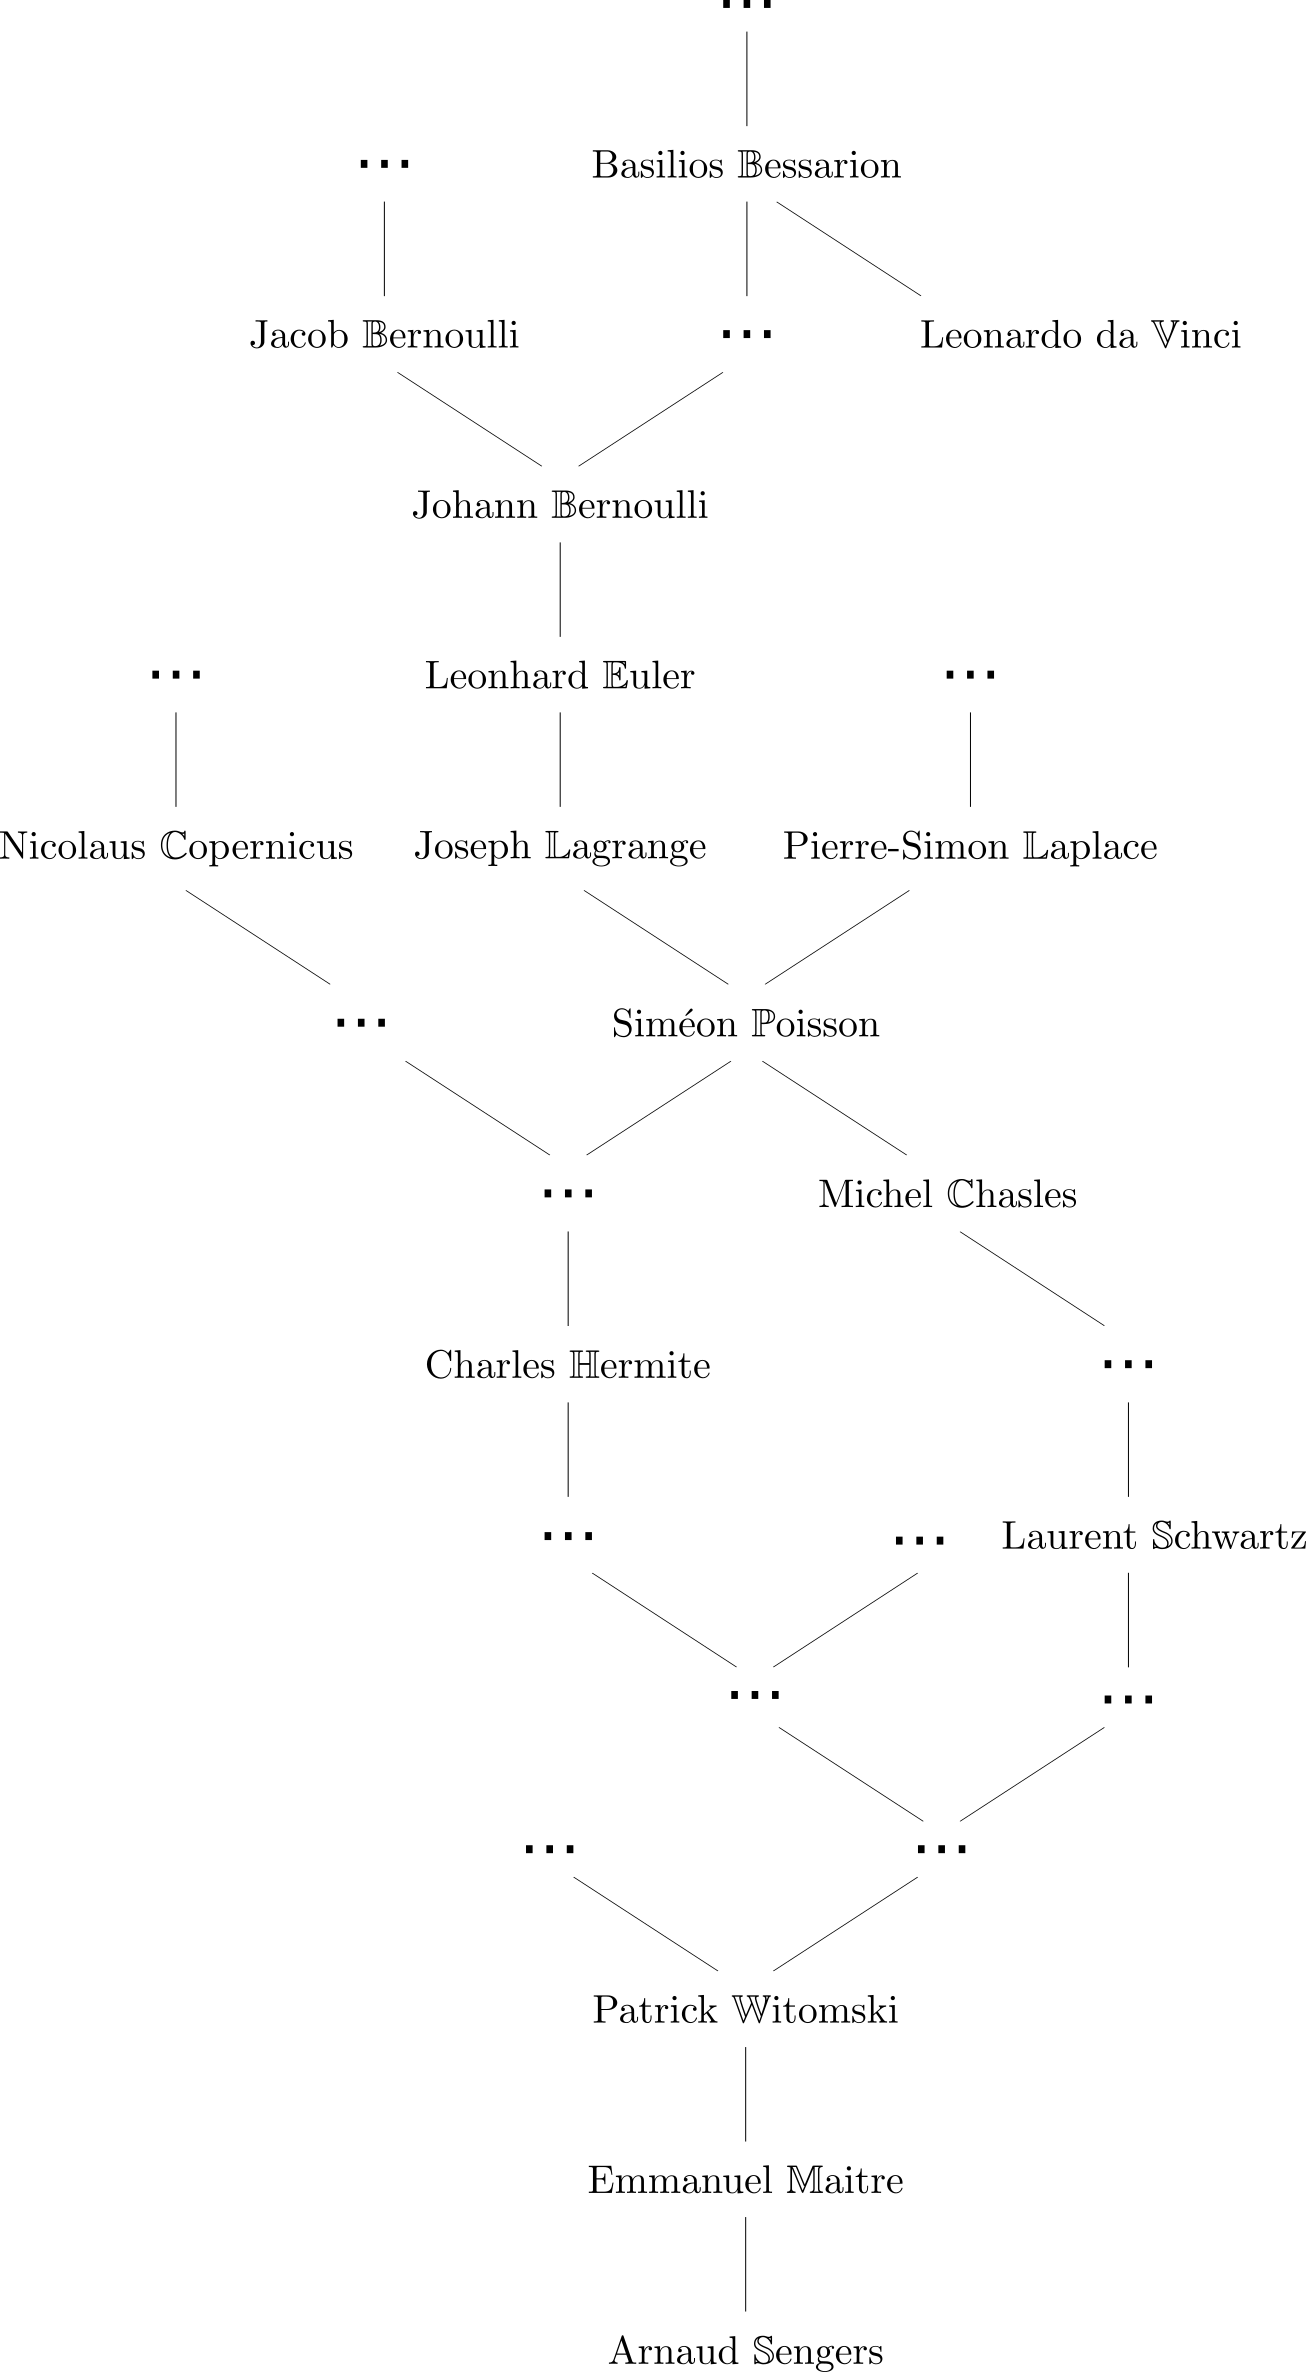
\includegraphics[width=\textwidth]{genealogie.png}
  \caption{Découvre tous les fameux ancêtres d'Arnaud}
\label{fig:genealogie}
\end{figure}


\section*{Le saviez-vous}
\begin{itemize}
\item Le séminaire des doctorants donné par Arnaud le mercredi 27/06/2018 a été celui qui a enregistré la plus grande affluence en 2 ans.
\item L'équipe de foot du LJK coachée par Arnaud a atteint les 8èmes de finales du tournoi inter-labos.
%\item Arnaud s'est un jour fait battre à la course à pied par un ancien doctorant, mais cela n'a jamais été vérifié % peut etre trop private joke
\item Arnaud possède une connaissance sommaire du latin et du grec ancien.
\end{itemize}


\section*{Loisirs}
Le temps peut parfois paraître un peu long durant cette demi-journée:
% \begin{itemize}
% \item Compter le nombre de fois que Arnaud dit \og essentiellement \fg: $\dots$
% \end{itemize}

%Compter le nombre de fois que Arnaud dit \og essentiellement \fg: $\dots$



\begin{table}[!h] % Idées bingo ?
  \centering
  \renewcommand{\arraystretch}{1.5}
  \begin{adjustbox}{tabular=*3{|c}|,center} \hline
    \og Instance \fg{} & Power pose & Pause boisson  \\ \hline
    Qqun s'endort & Case offerte!& Qqchose tombe \\ \hline
    Qqun en retard & Bruit de tablette & Chuchotements \\ \hline
  \end{adjustbox}
  \caption{Bingo}
\end{table}

\begin{figure}
	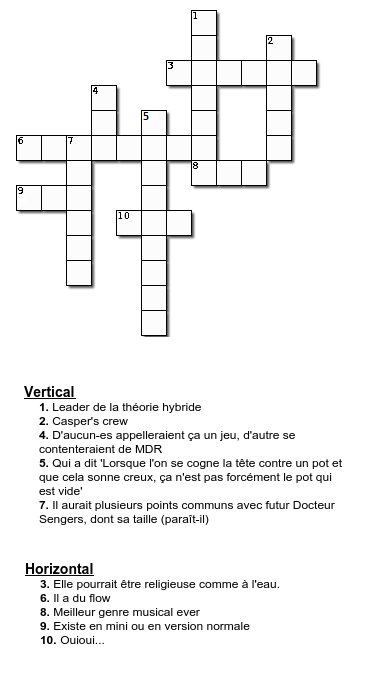
\includegraphics[width=\textwidth]{mots.png}
	\caption{Carrefour de mots.}
        \label{fig:carrouf}
\end{figure}

\end{document}



%%% Local Variables:
%%% mode: latex
%%% TeX-master: t
%%% End:
